\documentclass[11pt]{beamer}

\usetheme{CambridgeUS}
\usecolortheme{dolphin}

\usepackage[utf8]{inputenc}
\usepackage[L7x]{fontenc}
\usepackage[lithuanian]{babel}

\usepackage{amsmath}
\usepackage{amsfonts}
\usepackage{amssymb}
\usepackage{graphicx}


\usepackage{booktabs}
\usepackage{longtable}
\usepackage{array}
\usepackage{multirow}
\usepackage{wrapfig}
\usepackage{float}
\usepackage{colortbl}
\usepackage{pdflscape}
\usepackage{tabu}
\usepackage{threeparttable}
\usepackage{threeparttablex}
\usepackage[normalem]{ulem}
\usepackage{makecell}
\usepackage{xcolor}

\usepackage{hyperref}
\hypersetup{
  colorlinks=true,
  linkcolor=black,
  filecolor=blue,   
  urlcolor=blue,
  citecolor=blue
}

\author{Armintė G. Justas M. Tomas D.}
\title{COVID-19}
\subtitle{Skaičiai bei įžvalgos}
%\setbeamercovered{transparent} 
%\setbeamertemplate{navigation symbols}{} 
%\logo{} 
%\institute{Corona-Stat.lt} 
%\date{} 
%\subject{AAA} 

\graphicspath{{./figures/}}


\begin{document}

\begin{frame}
\titlepage
\end{frame}

\begin{frame}
\tableofcontents
\end{frame}

\section{Apie Corona-Stat.lt}
\begin{frame}{Corona-Stat.lt projektas}
\begin{itemize}
\item Corona-Stat.lt pirminis tikslas COVID19 plitimo prognozė
\item Komanda (Armintė, Rokas, Tomas)
\item SAM'o nulinė reakcija
\item Nuo COVID19 statistikos link ekonominių įžvalgų
\end{itemize}
\end{frame}


\begin{frame}{Apie COVID prognozavimą}
\begin{itemize}
\item Kaip prognozuojamos epi- ir pandemijos: SIR
\item $S \Longrightarrow I \Longrightarrow R$
\item Duomenų tikslumas (testavimo apimtis, latentinis periodas < inkubacinis periodas, asimptominis sirgimas, autopsijos)
\item \href{https://mif.vu.lt/lt3/dokumentai/dokumentai/Naujienos/COVID/2020-04-15_SEIR_ilgalakes_prognozes.pdf}{Lietuviški mokslininkai "prognozuoja"}
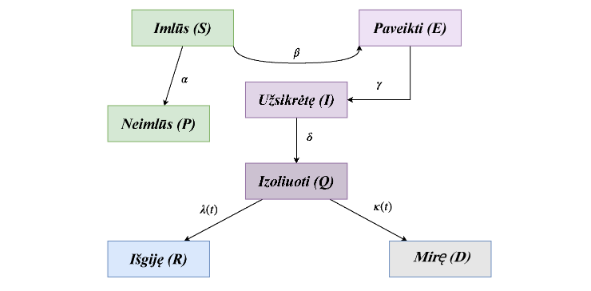
\includegraphics[scale=0.4]{seiqrdp.png}

\end{itemize}
\end{frame}

\section{Covid situacija}
\begin{frame}{Covid situacija}

\end{frame}


\begin{frame}{Apple maps užklausos}
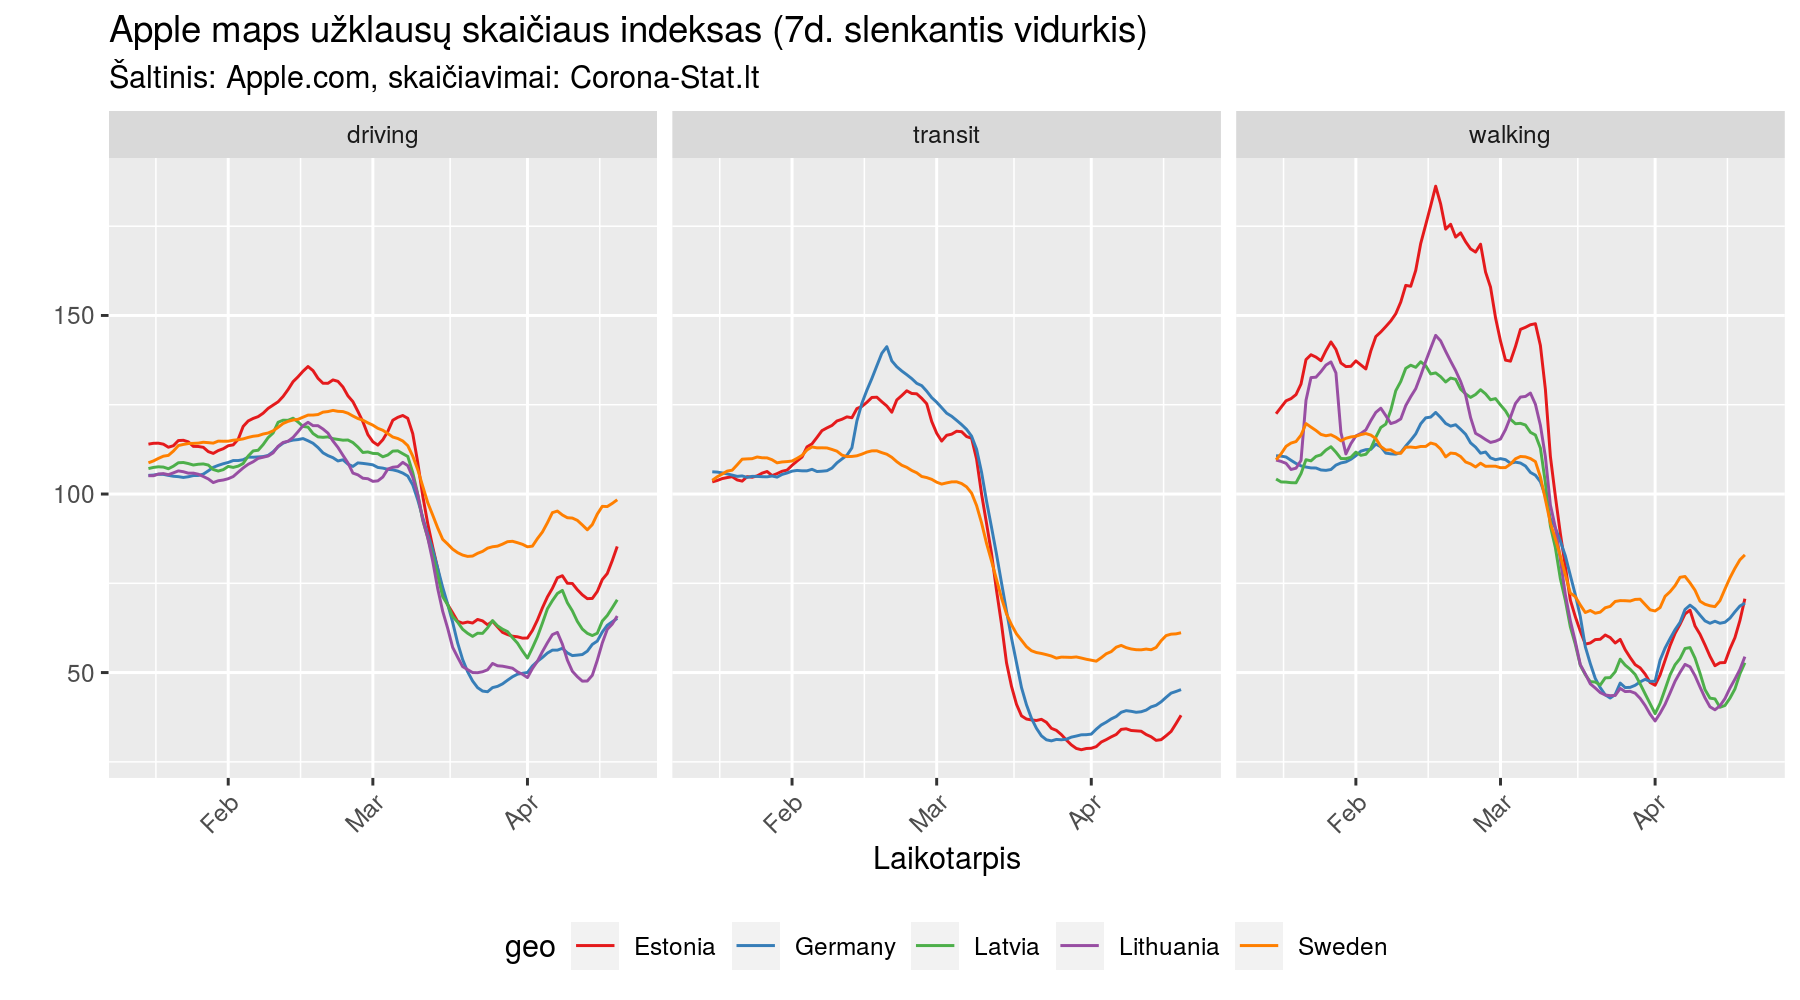
\includegraphics[scale=0.5]{apple_judejimas.png}
\end{frame}

\begin{frame}{Apple maps užklausos}
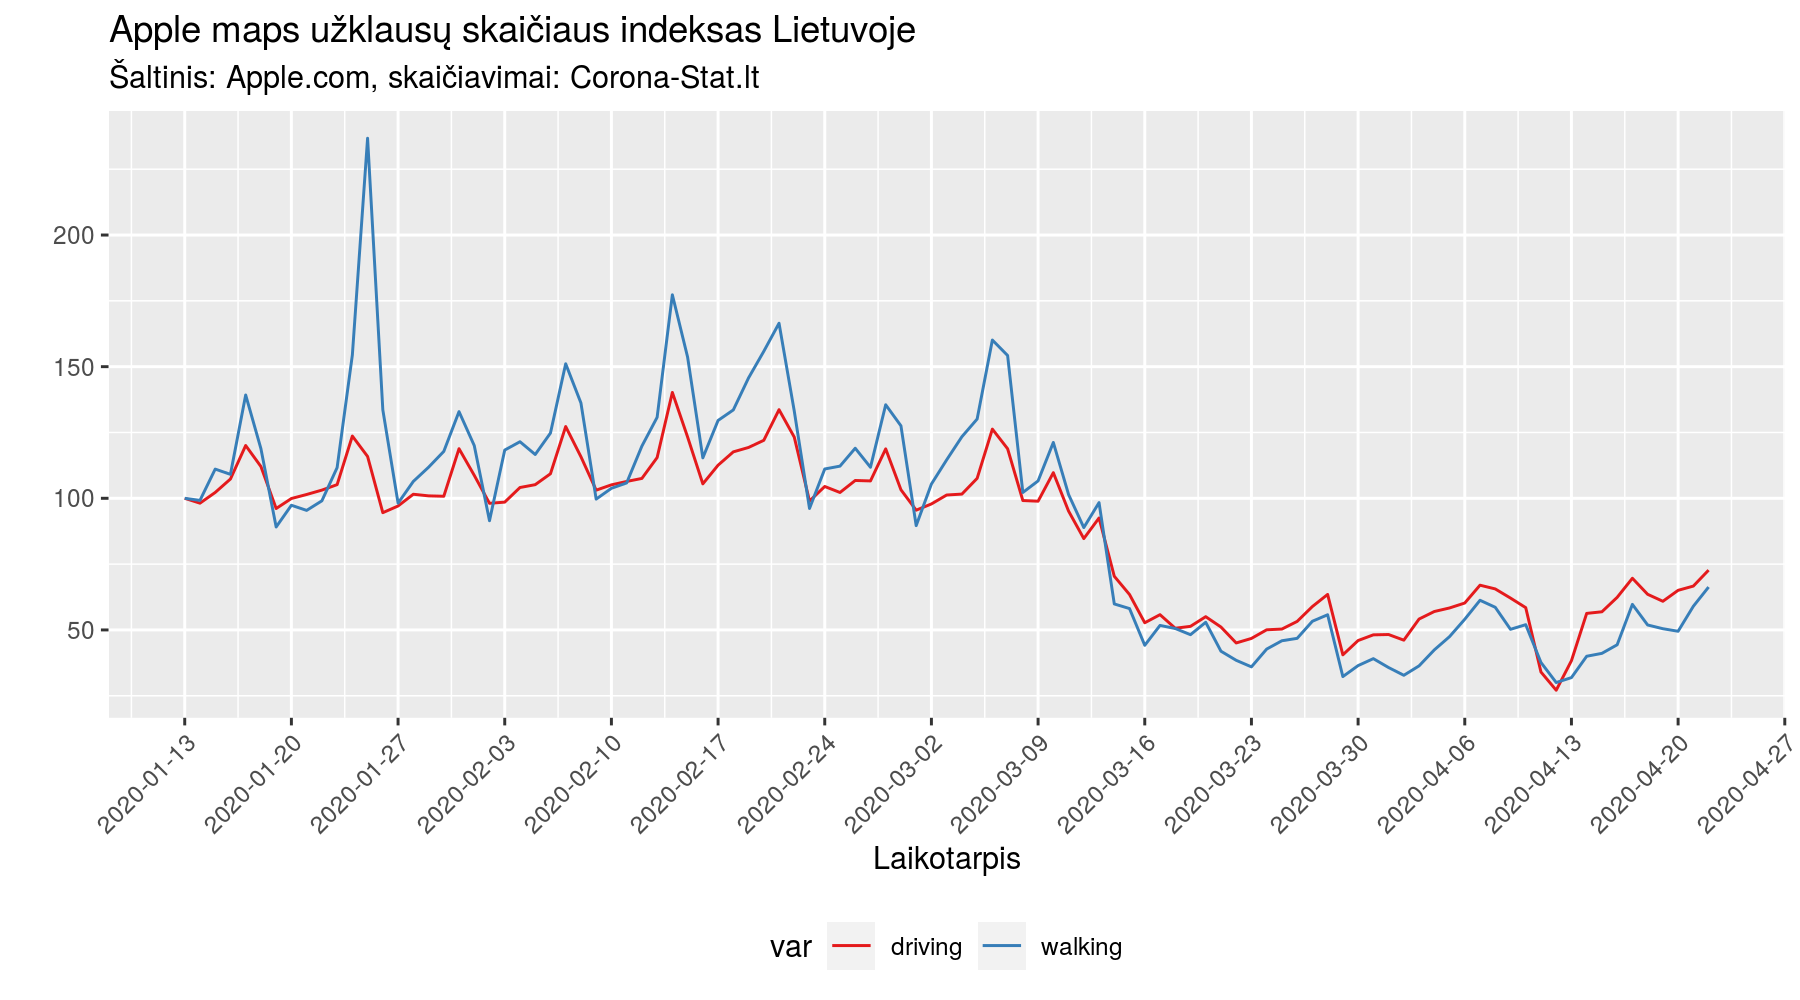
\includegraphics[scale=0.5]{apple_judejimas_lt.png}
\end{frame}

\section{Nedarbas Lietuvoje}

\begin{frame}{Grupės darbuotojų atleidimai}
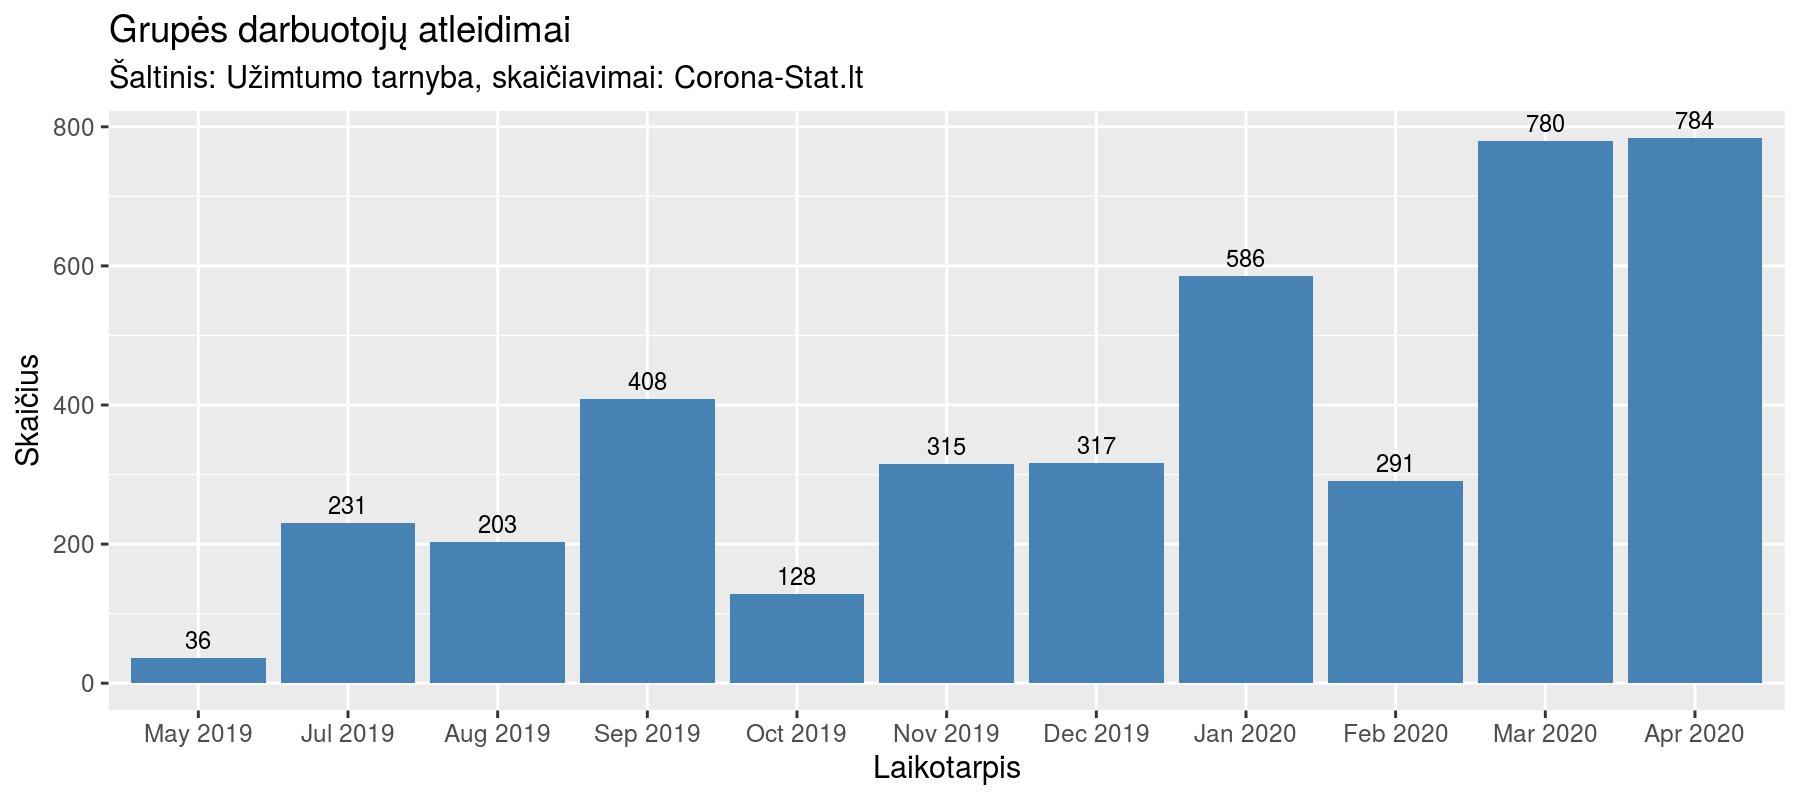
\includegraphics[scale=0.5]{grupes_darbuotoju_atleidimai_men_sum.png}
\begin{footnotesize}
\begin{itemize}
\item Keleivinis oro transportas	420
\item Drabužiai + avalynė 239
\item Baldų gamyba	87
\item Konsultacinė verslo veikla	83
\end{itemize}
\end{footnotesize}
\end{frame}


%\begin{frame}{Grupės darbuotojų atleidimai}
%Grupės darbuotojų atleidimai nuo 2020 vasario mėn.
%\input{grupiniai_atleidimai.txt}
%\end{frame}

\begin{frame}{Bedarbių skaičius}
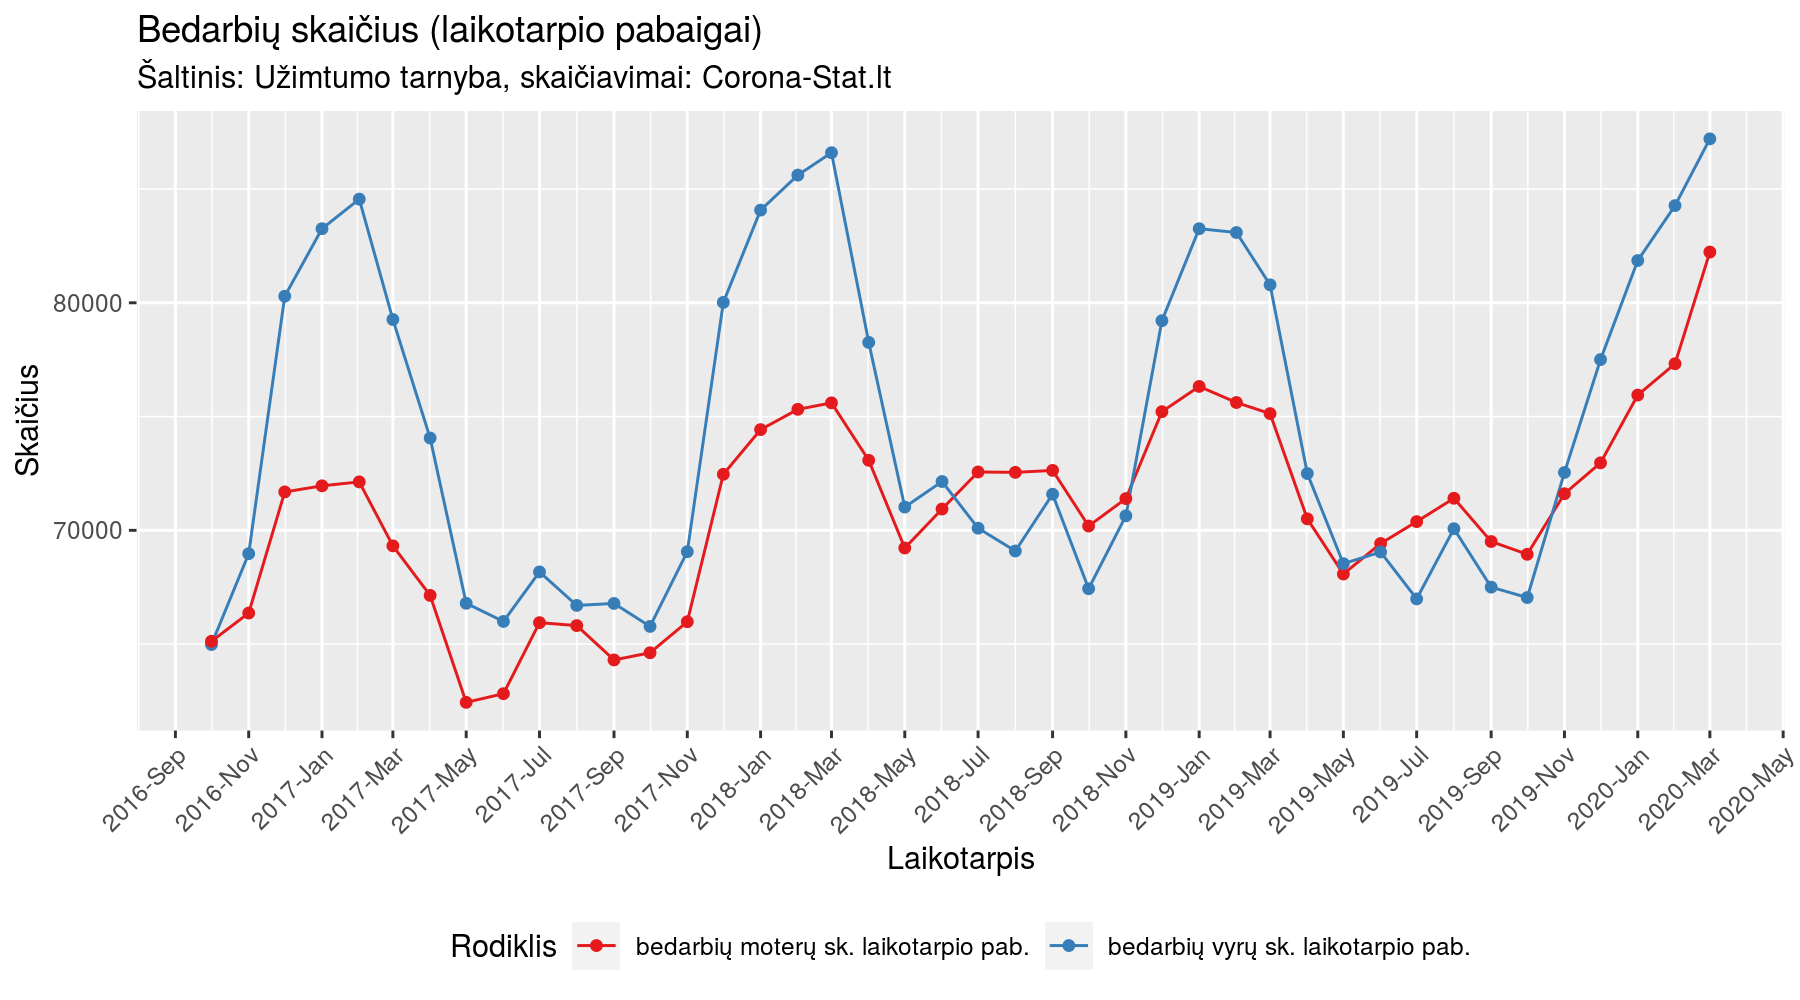
\includegraphics[scale=0.5]{bedarbiu_sk.png}
\end{frame}

%\begin{frame}{Bedarbių proc. nuo DAG}
%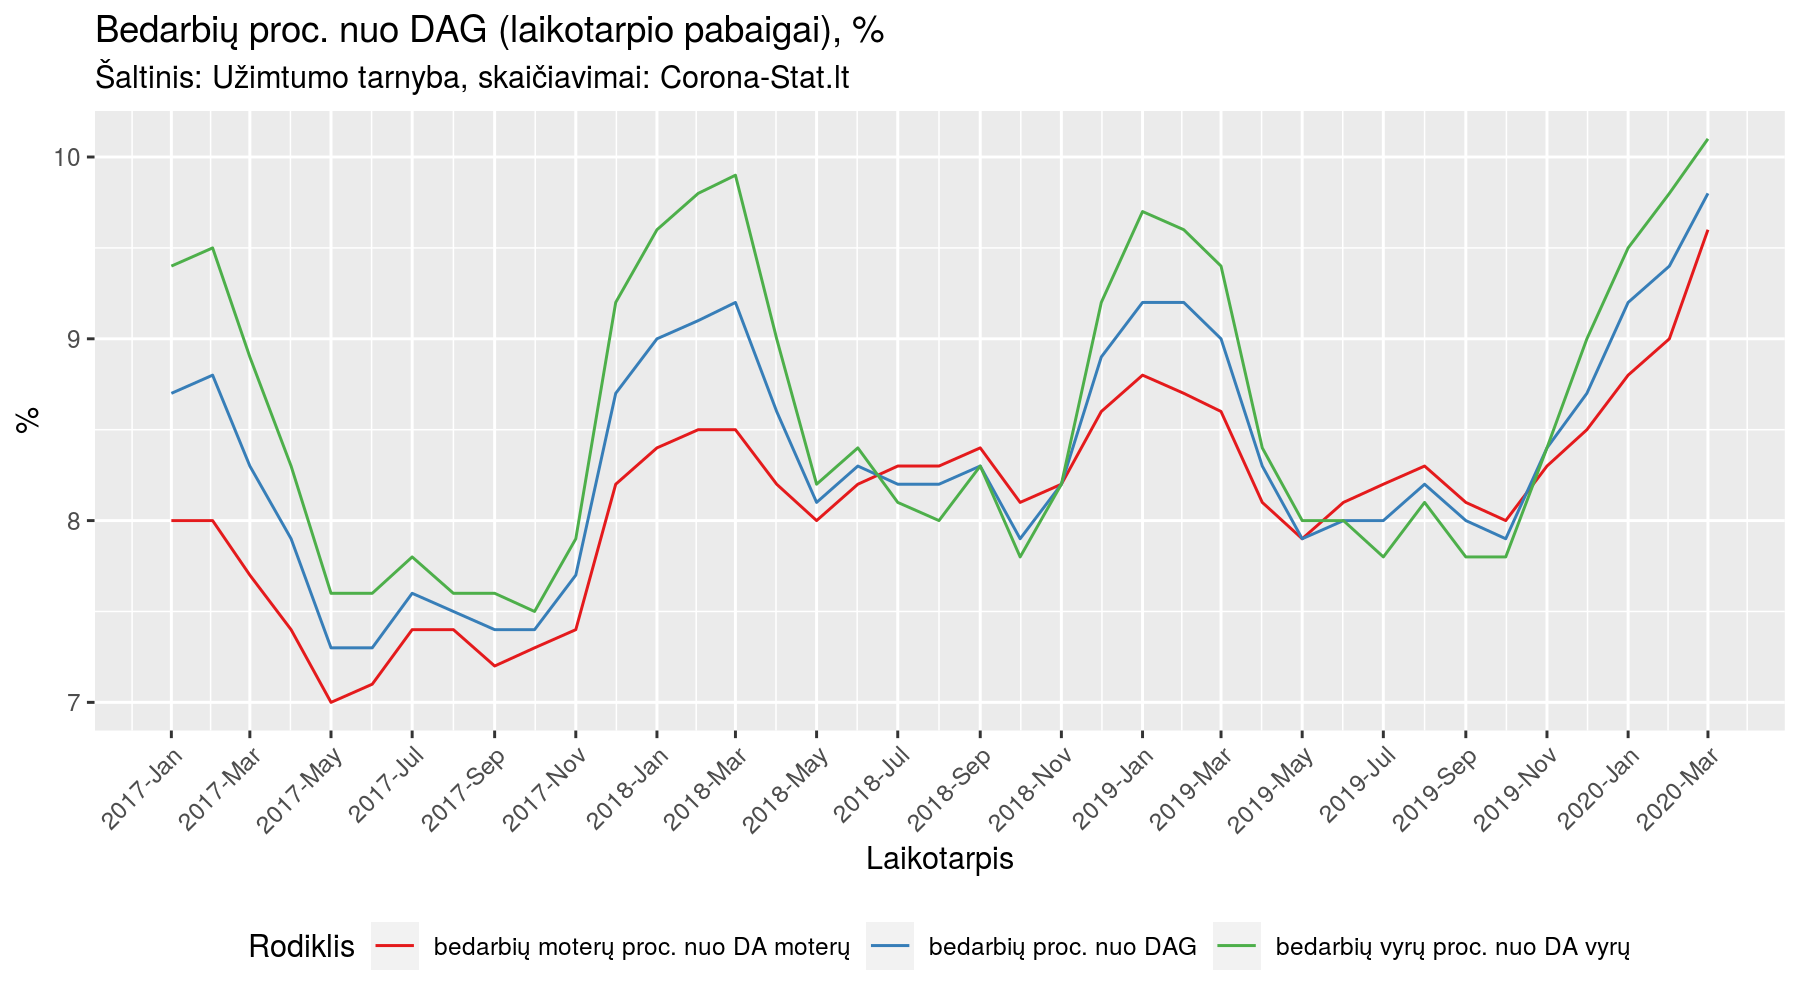
\includegraphics[scale=0.5]{bedarbiu_proc.png}
%\end{frame}




\section{Infliacija}
\begin{frame}{Eurozonos metinė infliacija}
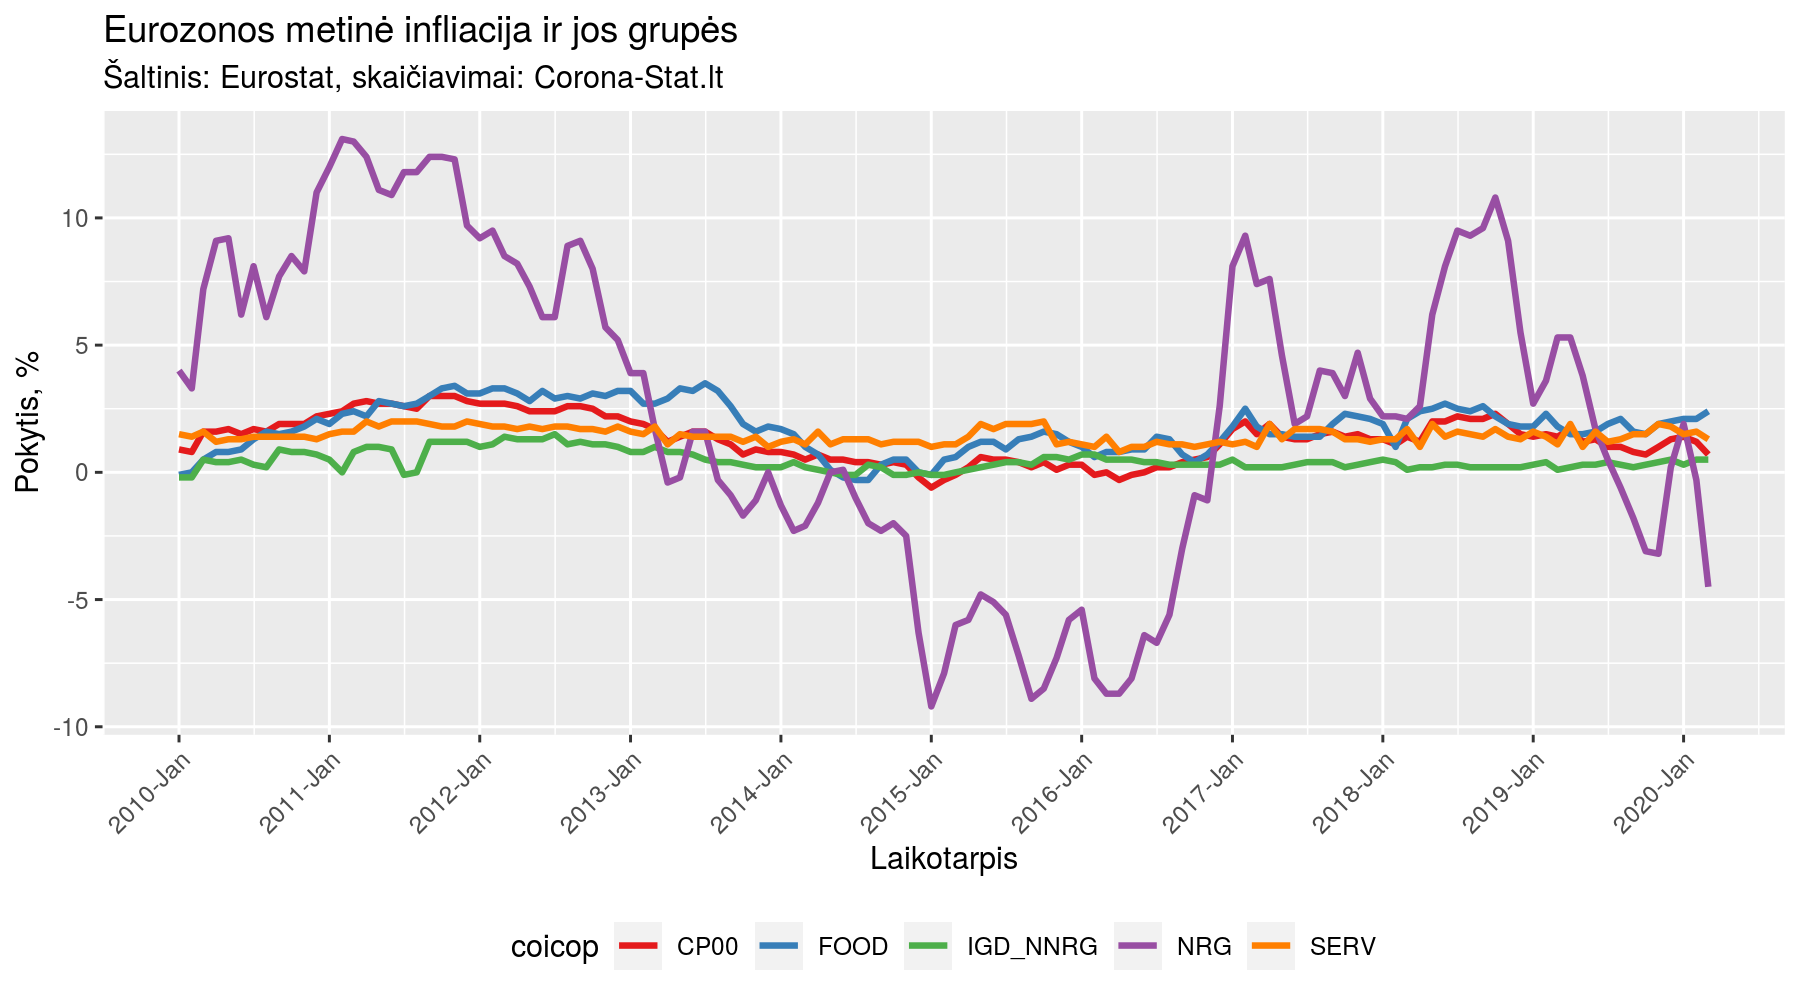
\includegraphics[scale=0.5]{infliacija_ez.png}
\end{frame}

\begin{frame}{Eurozonos metinė infliacija}
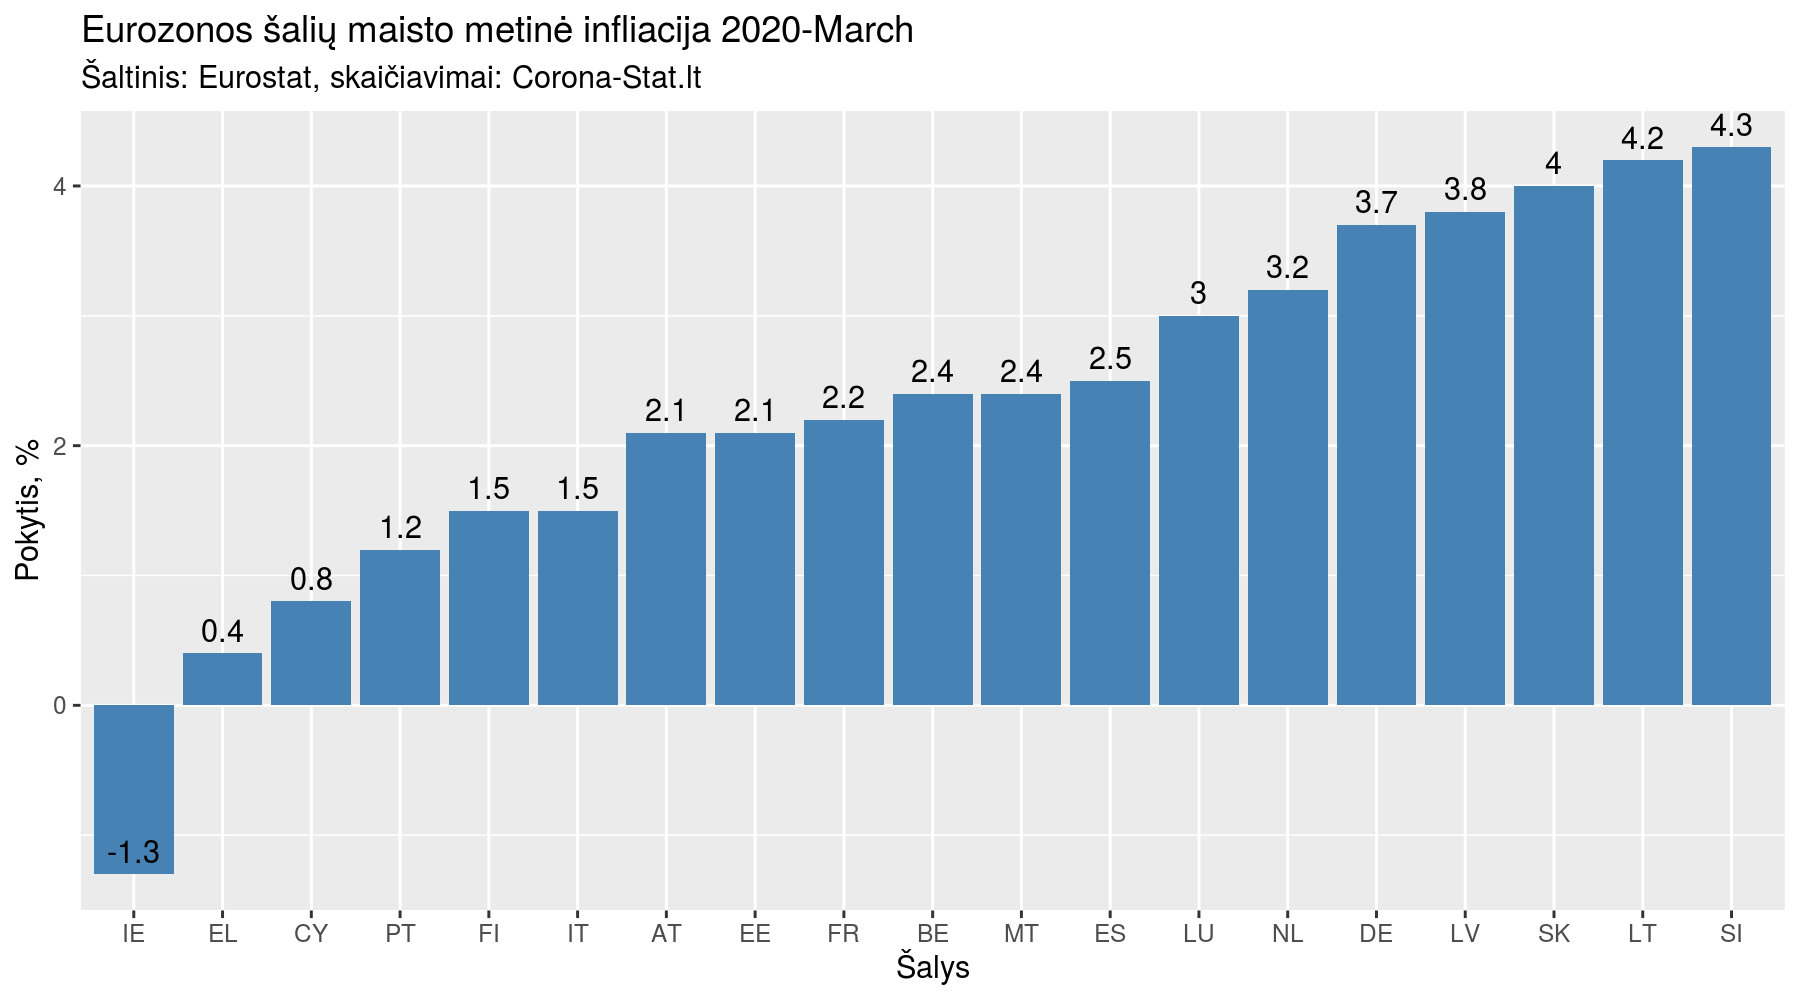
\includegraphics[scale=0.5]{infliacija_maistas.png}
\end{frame}

\begin{frame}{Eurozonos metinė infliacija}
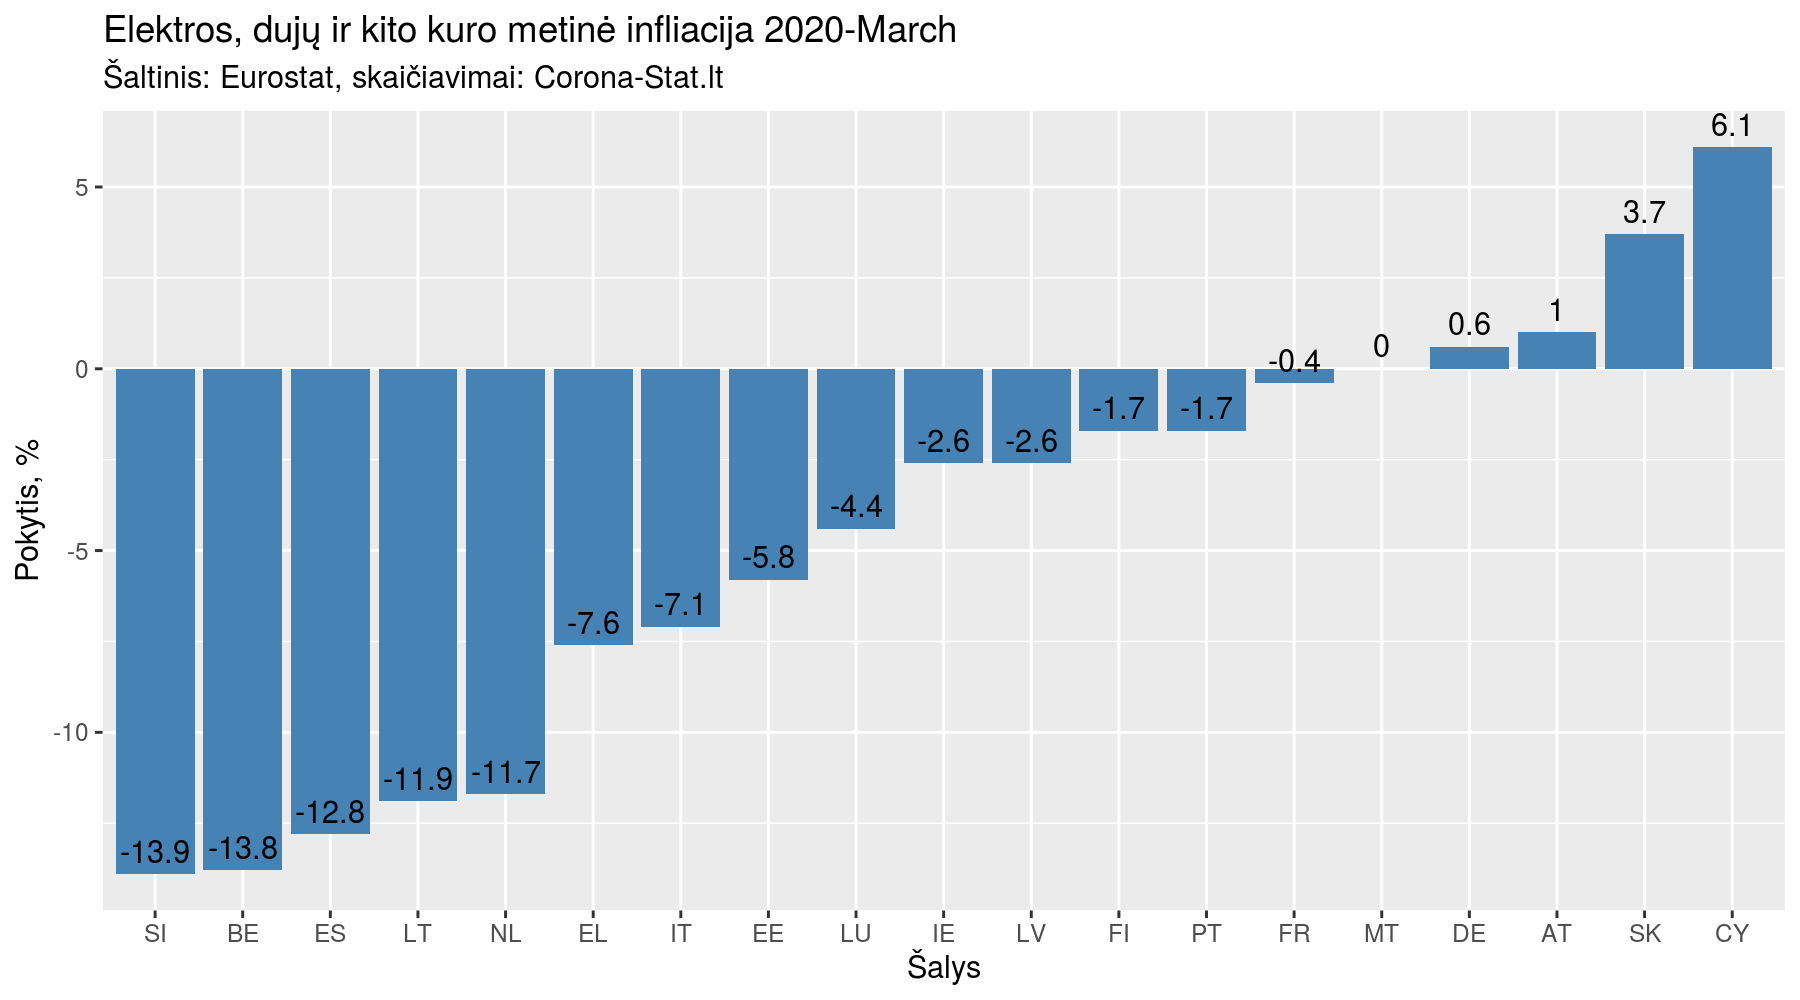
\includegraphics[scale=0.5]{infliacija_elektra_dujos.png}
\end{frame}


\begin{frame}{Eurozonos metinė infliacija}
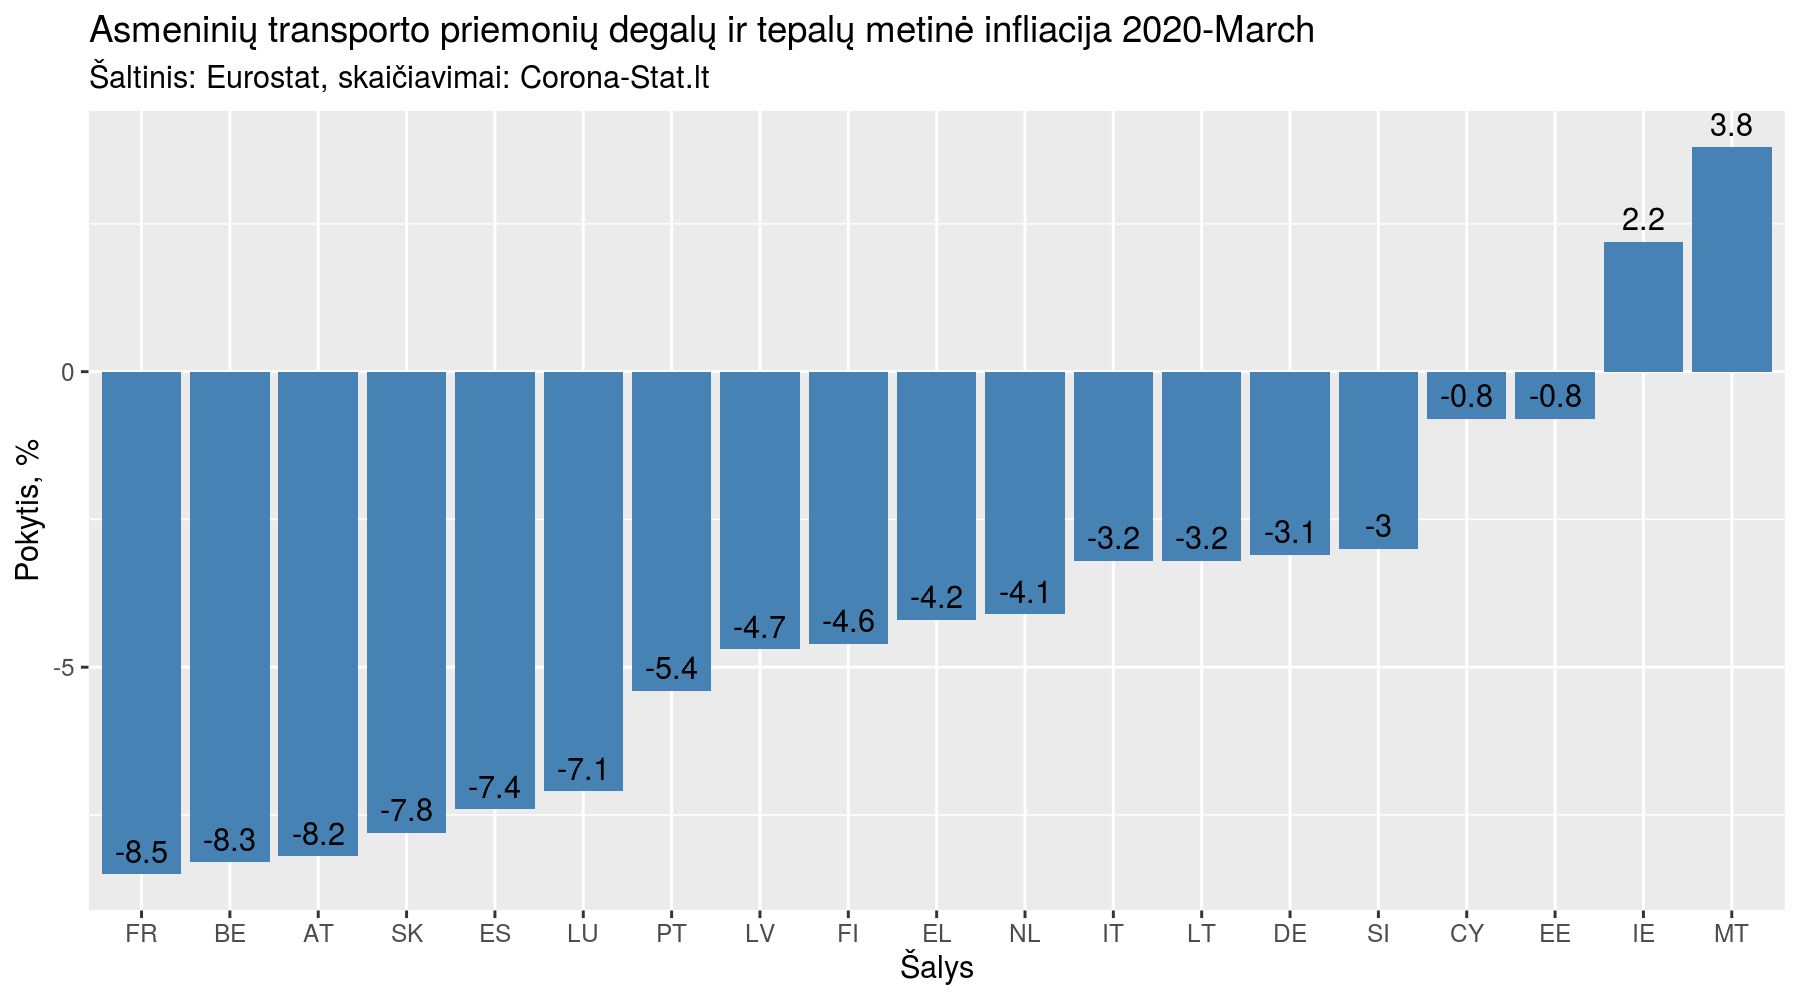
\includegraphics[scale=0.5]{infliacija_degalai.png}
\end{frame}



\section{Pramonė, lūkesčiai, eksporto rinkos}

\begin{frame}{Lietuva maža ir atvira ekonomika}
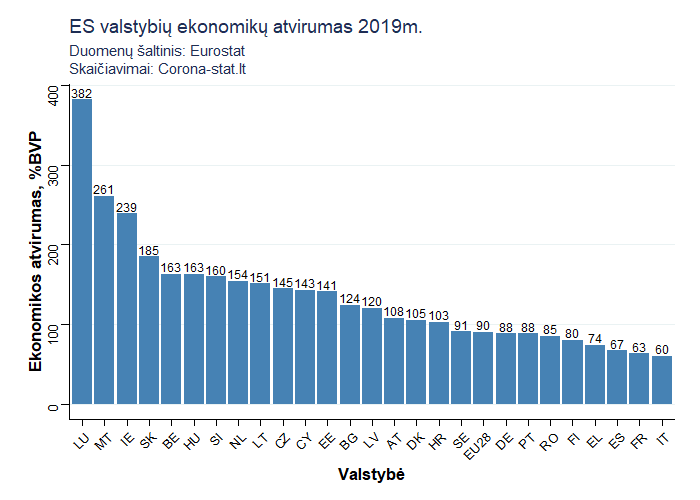
\includegraphics[scale=0.5]{atvirumas.png}
\end{frame}



\begin{frame}{Verlso lūkesčiai kaip vedantieji (lead) inkdikatoriai}
\begin{scriptsize}
\end{scriptsize}
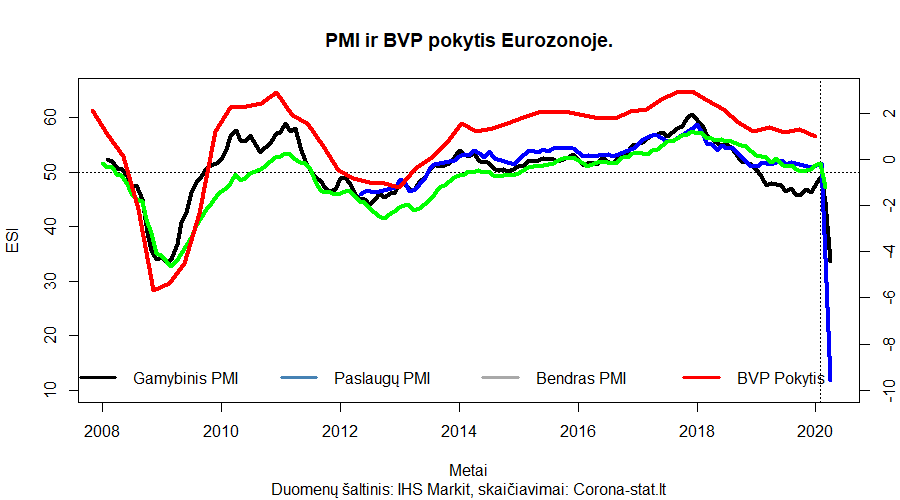
\includegraphics[scale=0.5]{Rplot05.png}
\end{frame}

\begin{frame}{Nepaisant milžiniškų skatinimo paketų...}
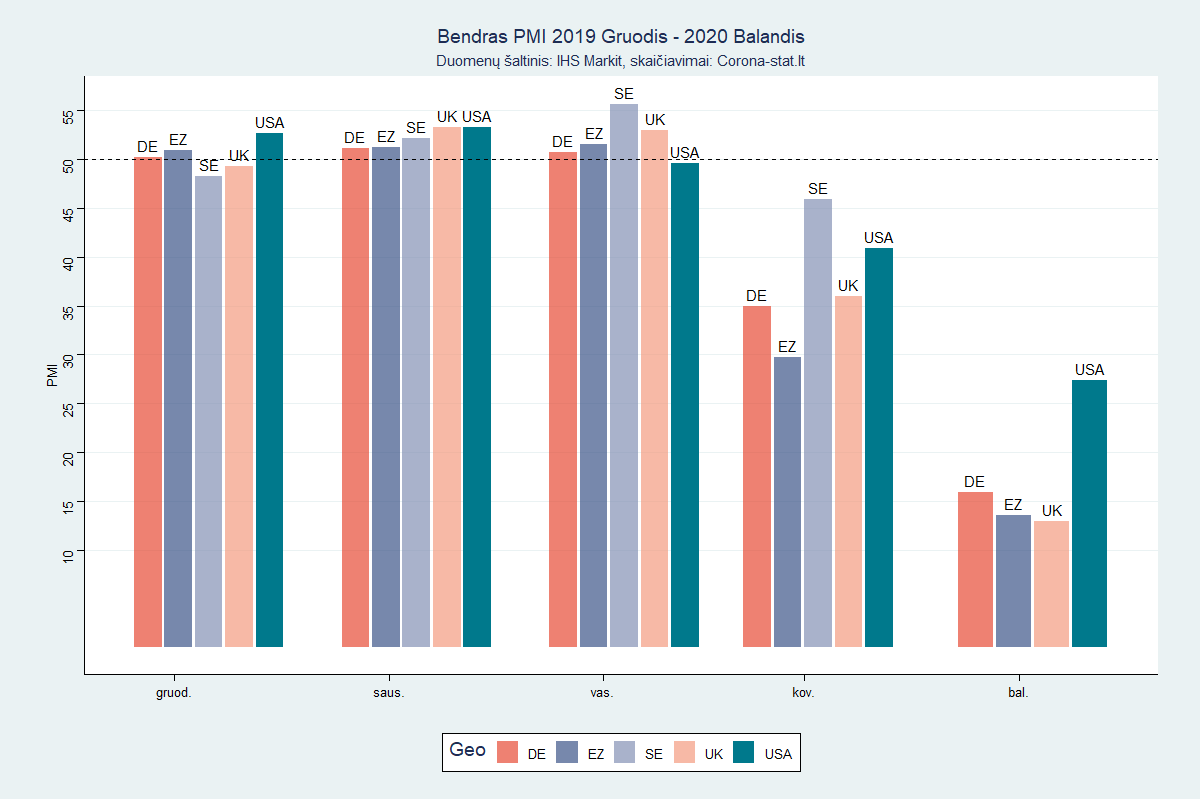
\includegraphics[scale=0.3]{tomas_1.png}
\end{frame}

\begin{frame}{Situacija Lietuvoje}
\begin{itemize}
\item 
\item 
\item 
\end{itemize}
\end{frame}



\section{Kodėl krenta naftos kaina?}

\begin{frame}{Naftos paklausa ir karas dėl Kinijos}
Naftos rinka – dviguboje krizėje:
\begin{itemize}
\item Dėl stojančios ekonomikos mažėja pasaulinė naftos paklausa
\begin{itemize}
\item Naftos paklausa ir pasiūla yra neelastinga kainos atžvilgiu
\end{itemize}
\item Tarp naftos gavybos šalių prasidėjo karas dėl ateities rinkų
\begin{itemize}
\item Trump bandymas inicijuoti gavybos mažinimą
\item Saudo Arabijos ir Rusijos kainų karas
\item Didžiausias laimėtojas - Kinija
\item Balandžio 12d. OPEC+ susitarė dėl 9.7 mln barelių (~10 proc. visos gavybos)
\end{itemize}
\end{itemize}
\end{frame}


\begin{frame}{Naftos kaina ir jos poveikis geopolitikai}
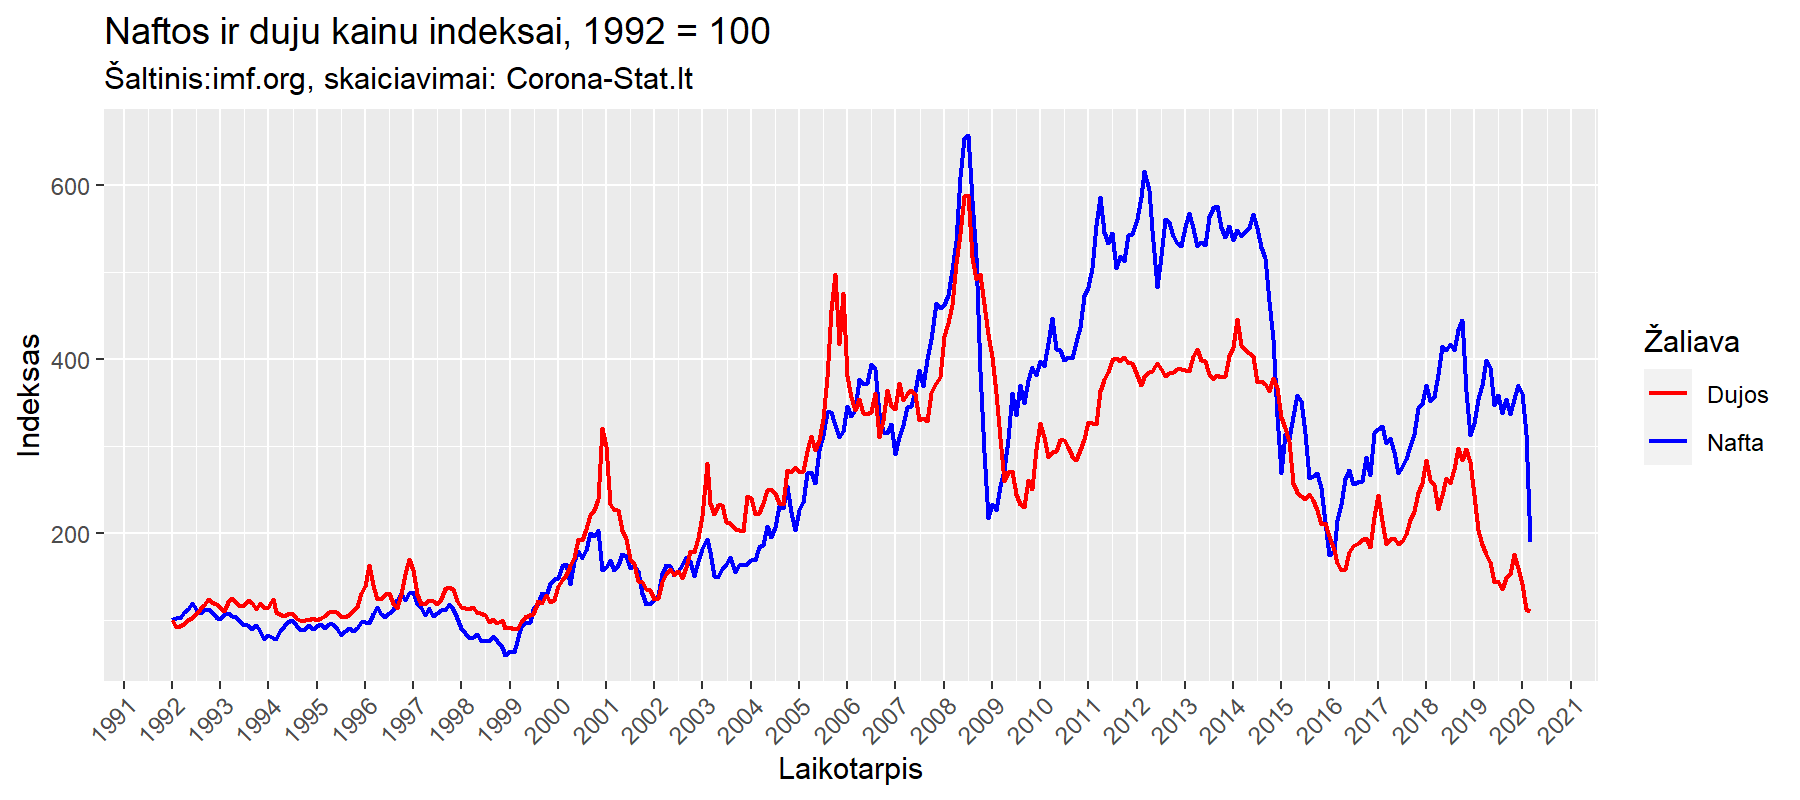
\includegraphics[scale=0.5]{naftos_kainos_monthly.png}
\end{frame}

\begin{frame}{WTI spekuliacijos burbulo sprogimas}
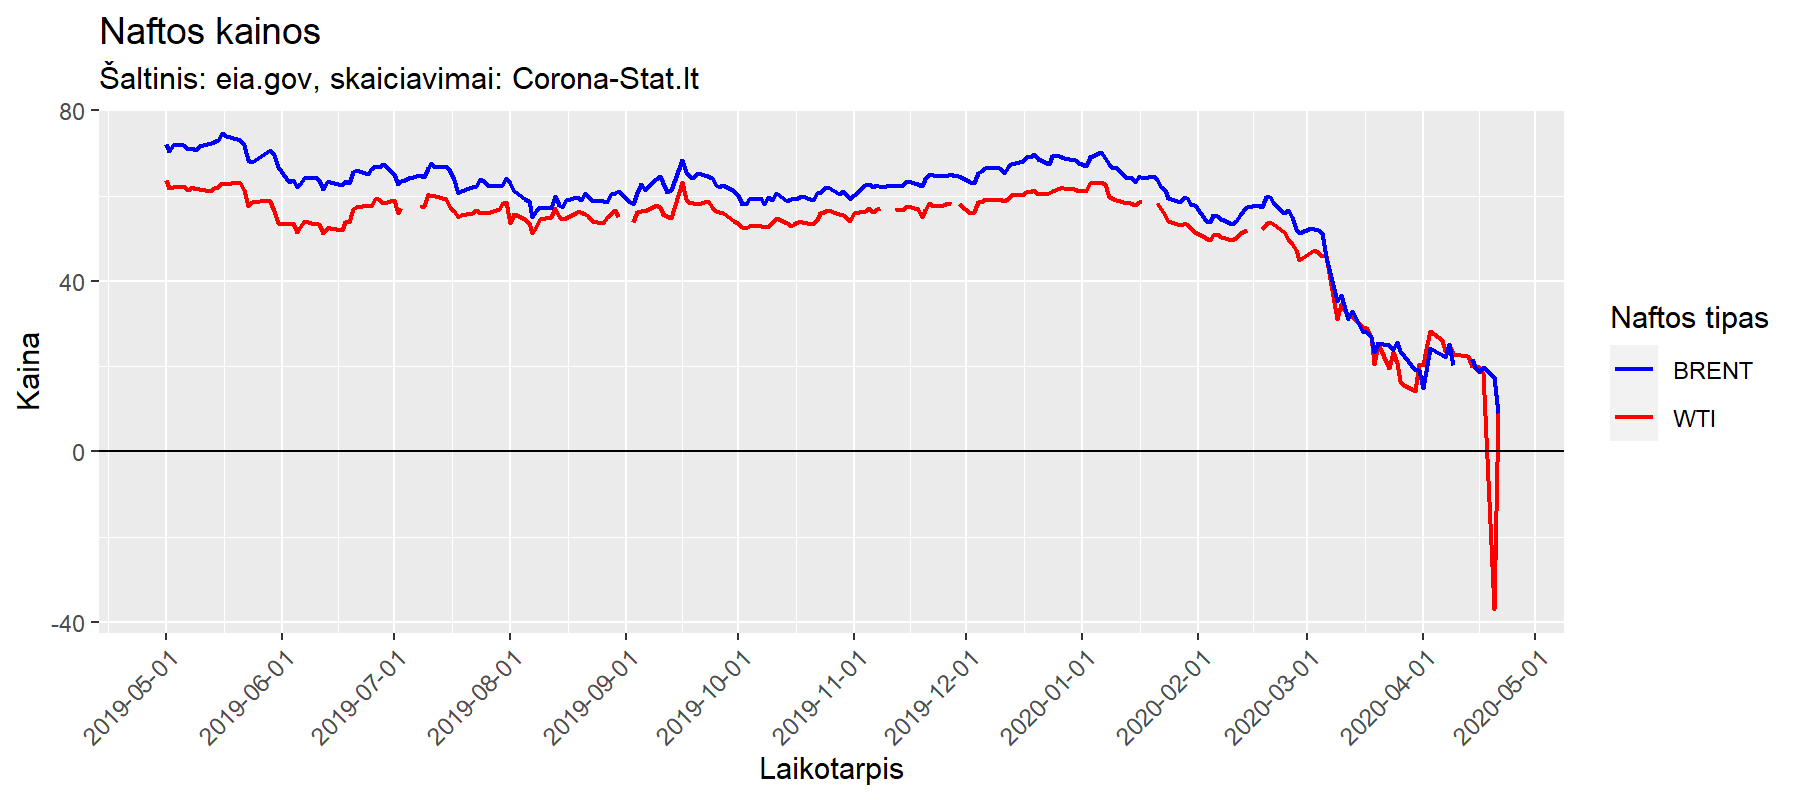
\includegraphics[scale=0.5]{naftos_kainos_daily.png}
\end{frame}

\begin{frame}{Naftos kainų poveikis}
Lietuvoje:
\begin{itemize}
\item Elektra planuojama atpigs 22 \%
\item Dujos namų ūkiams - 15-22 \%
\item Bendras kainų mažėjimas. (pvz., maisto produktų)
\item Sąlyginė pagalba Achemai - didžiausiai pramoninei dujų vartotojai Lietuvoje
\end{itemize}
Globaliai:
\begin{itemize}
\item mažesnės investicijos į atsinaujinančią energetiką
\item galimai keistis ES MFF prioritetai (mažiau Green Deal)
\item galimos didesnės geopolitinės įtampos (pvz., Rusija)
\item dar mažiau JAV dėmesio Artimiesiems rytams ir daugiau dėmesio Pietryčių Azijai
\end{itemize}
\end{frame}


\section{Koronabonds}

\begin{frame}{Ar COVID19 sugriaus Europą?}
Kodėl coronabonds o ne ESM
\end{frame}

\begin{frame}{Ar COVID19 sugriaus Europą?}
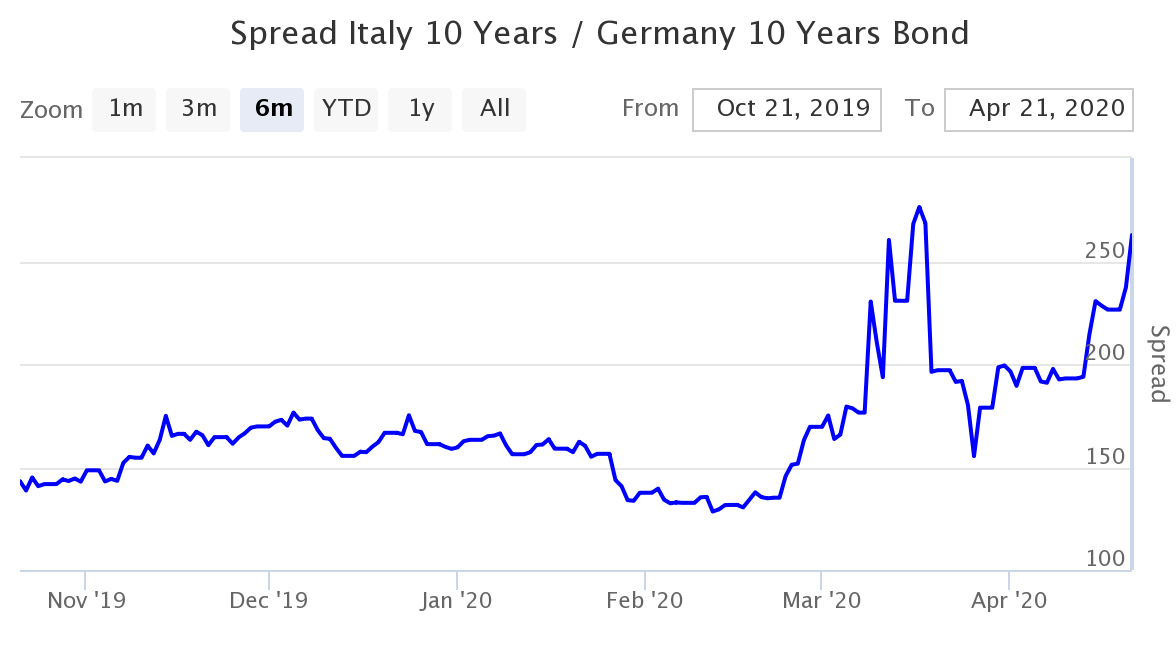
\includegraphics[scale=0.25]{spread-italy-10-years-ge.png}
http://www.worldgovernmentbonds.com/spread/italy-10-years-vs-germany-10-years/
\end{frame}

\end{document}